

\tikzset{every picture/.style={line width=0.75pt}} %set default line width to 0.75pt        

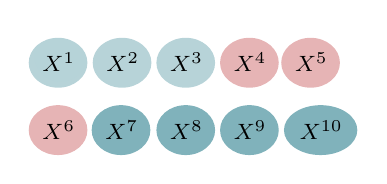
\begin{tikzpicture}[x=0.75pt,y=0.75pt,yscale=-1,xscale=1]
%uncomment if require: \path (0,293); %set diagram left start at 0, and has height of 293

%Shape: Circle [id:dp1678818803252513] 
\draw  [draw opacity=0][fill={rgb, 255:red, 255; green, 255; blue, 255 }  ,fill opacity=1 ] (64.21,98.63) .. controls (64.05,91.62) and (69.6,85.8) .. (76.62,85.64) .. controls (83.63,85.47) and (89.45,91.03) .. (89.61,98.04) .. controls (89.77,105.06) and (84.22,110.88) .. (77.2,111.04) .. controls (70.19,111.2) and (64.37,105.65) .. (64.21,98.63) -- cycle ;

% Text Node
\draw  [draw opacity=0][fill={rgb, 255:red, 206; green, 106; blue, 107 }  ,fill opacity=0.5 ]  (167.86, 101.87) circle [x radius= 14.14, y radius= 12.02]   ;
\draw (158.86,95.77) node [anchor=north west][inner sep=0.75pt]  [font=\footnotesize]  {$X^{4}$};
% Text Node
\draw  [draw opacity=0][fill={rgb, 255:red, 74; green, 145; blue, 158 }  ,fill opacity=0.4 ]  (75.67, 101.87) circle [x radius= 14.14, y radius= 12.02]   ;
\draw (66.67,95.77) node [anchor=north west][inner sep=0.75pt]  [font=\footnotesize]  {$X^{1}$};
% Text Node
\draw  [draw opacity=0][fill={rgb, 255:red, 206; green, 106; blue, 107 }  ,fill opacity=0.5 ]  (197.33, 101.87) circle [x radius= 14.14, y radius= 12.02]   ;
\draw (188.33,95.77) node [anchor=north west][inner sep=0.75pt]  [font=\footnotesize]  {$X^{5}$};
% Text Node
\draw  [draw opacity=0][fill={rgb, 255:red, 74; green, 145; blue, 158 }  ,fill opacity=0.4 ]  (137.19, 101.87) circle [x radius= 14.14, y radius= 12.02]   ;
\draw (128.19,95.77) node [anchor=north west][inner sep=0.75pt]  [font=\footnotesize]  {$X^{3}$};
% Text Node
\draw  [draw opacity=0][fill={rgb, 255:red, 74; green, 145; blue, 158 }  ,fill opacity=0.4 ]  (106.5, 101.87) circle [x radius= 14.14, y radius= 12.02]   ;
\draw (97.5,95.77) node [anchor=north west][inner sep=0.75pt]  [font=\footnotesize]  {$X^{2}$};
% Text Node
\draw  [draw opacity=0][fill={rgb, 255:red, 206; green, 106; blue, 107 }  ,fill opacity=0.5 ]  (75.67, 134.32) circle [x radius= 14.14, y radius= 12.02]   ;
\draw (66.67,128.22) node [anchor=north west][inner sep=0.75pt]  [font=\footnotesize]  {$X^{6}$};
% Text Node
\draw  [draw opacity=0][fill={rgb, 255:red, 74; green, 145; blue, 158 }  ,fill opacity=0.7 ]  (106, 134.32) circle [x radius= 14.14, y radius= 12.02]   ;
\draw (97,128.22) node [anchor=north west][inner sep=0.75pt]  [font=\footnotesize]  {$X^{7}$};
% Text Node
\draw  [draw opacity=0][fill={rgb, 255:red, 74; green, 145; blue, 158 }  ,fill opacity=0.7 ]  (137.19, 134.32) circle [x radius= 14.14, y radius= 12.02]   ;
\draw (128.19,128.22) node [anchor=north west][inner sep=0.75pt]  [font=\footnotesize]  {$X^{8}$};
% Text Node
\draw  [draw opacity=0][fill={rgb, 255:red, 74; green, 145; blue, 158 }  ,fill opacity=0.7 ]  (167.86, 134.32) circle [x radius= 14.14, y radius= 12.02]   ;
\draw (158.86,128.22) node [anchor=north west][inner sep=0.75pt]  [font=\footnotesize]  {$X^{9}$};
% Text Node
\draw  [draw opacity=0][fill={rgb, 255:red, 74; green, 145; blue, 158 }  ,fill opacity=0.7 ]  (202.18, 134.32) circle [x radius= 17.68, y radius= 12.02]   ;
\draw (190.68,128.22) node [anchor=north west][inner sep=0.75pt]  [font=\footnotesize]  {$X^{10}$};


\end{tikzpicture}
